\documentclass{beamer}
%Для защит онлайн лучше использовать разрешение 16x9
%\documentclass[aspectratio=169]{beamer}

%%% Обязательные пакеты
%% Beamer
\usepackage{beamerthemesplit}
\usetheme{SPbGU}
\beamertemplatenavigationsymbolsempty
\usepackage{appendixnumberbeamer}

%% Локализация
\usepackage{fontspec}
\setmainfont{CMU Serif}
\setsansfont{CMU Sans Serif}
\setmonofont{CMU Typewriter Text}
%\setmonofont{Fira Code}[Contextuals=Alternate,Scale=0.9]
%\setmonofont{Inconsolata}
% \newfontfamily\cyrillicfont{CMU Serif}

\usepackage{polyglossia}
\setdefaultlanguage{russian}
\setotherlanguage{english}
\usepackage[autostyle]{csquotes} % Правильные кавычки в зависимости от языка

%% Графика
\usepackage{wrapfig} % Позволяет вставлять графику, обтекаемую текстом
\usepackage{pdfpages} % Позволяет вставлять многостраничные pdf документы в текст

%% Математика
\usepackage{amsmath, amsfonts, amssymb, amsthm, mathtools} % "Адекватная" работа с математикой в LaTeX

% Математические окружения с русским названием
\newtheorem{rutheorem}{Теорема}
\newtheorem{ruproof}{Доказательство}
\newtheorem{rudefinition}{Определение}
\newtheorem{rulemma}{Лемма}


%%% Дополнительные пакеты. Используются в презентации, но могут быть отключены при необходимости
\usepackage{tikz} % Мощный пакет для создание рисунков, однако может очень сильно замедлять компиляцию
\usetikzlibrary{decorations.pathreplacing,calc,shapes,positioning,tikzmark}

\usepackage{multirow} % Ячейка занимающая несколько строк в таблице

%% Пакеты для оформления алгоритмов на псевдокоде
\usepackage[noend]{algpseudocode}
\usepackage{algorithm}
\usepackage{algorithmicx}

\usepackage{fancyvrb}

%% Пакет для анимированных иллюстраций
\usepackage{animate}


% То, что в квадратных скобках, отображается внизу по центру каждого слайда.
\title[Tokio global queue]{Оптимизация алгоритмов injected queue в
рантайме Tokio}

% То, что в квадратных скобках, отображается в левом нижнем углу.
\institute[СПбГУ]{}

% То, что в квадратных скобках, отображается в левом нижнем углу.
\author[Игорь Ерин]{Игорь Антонович Ерин, группа 21.Б10-мм}

\begin{document}
{
\setbeamertemplate{footline}{}
% Лого университета или организации, отображается в шапке титульного листа
\begin{frame}
  
\includegraphics[width=1.4cm]{pictures/SPbGU_Logo.png}
\vspace{-35pt}
\hspace{-10pt}
\begin{center}
   \begin{tabular}{c}
        \scriptsize{Санкт-Петербургский государственный университет} \\
        \scriptsize{Кафедра системного программирования}
    \end{tabular}
\titlepage
\end{center}

\btVFill

{\scriptsize
  % У научного руководителя должна быть указана научная степень
   \textbf{Научный руководитель:} к.ф.-м.н. В. И. Гориховский, доцент кафедры системного программирования \\
  % Консультанта может и не быть. Должна быть указана должность или ученая степень
   \textbf{Консультант:}  Р. С. Ефремов, программист ЗАО \enquote{Эксперт по разработке ПО, ООО ``Ядро Центр Программных Разработок''}\\
  % Для курсовой не обязателен. Должна быть указана должность или ученая степень
  %  \textbf{Рецензент:} д.т.н., проф. И.И. Иванов, исполнительный директор ООО \enquote{Рога и копыта}
 }
\begin{center}
  \vspace{5pt}
  \scriptsize{Санкт-Петербург\\
                 2025}
  \end{center}

\end{frame}
}

\begin{frame}[fragile]
  \frametitle{Введение}
  \begin{itemize}
    \item \verb|TATLIN.BACKUP|\footnote{\href{https://yadro.com/ru/tatlin/backup}{TATLIN.BACKUP} --- официальный сайт проекта (Дата обращения: 4.1.2025)} --- системы бекапов на \verb|Rust|
    \item Rust --- язык программирования общего назначения
    \begin{itemize}
      \item \verb|async| / \verb|await| интерфейс
      \item не фиксирует реализацию асинхронного рантайма
    \end{itemize}
    \item \verb|tokio|\footnote{\href{https://tokio.rs/}{tokio} --- официальный сайт проекта (Дата обращения: 4.1.2025)} --- проект используемый в \verb|TATLIN.BACKUP|
    \begin{itemize}
      \item рантаймы --- \verb|current_thread|, \verb|multi_thread|
      \item стандартную библиотеку языка с асинхронным интерфейсом
      \item примитивы синхронизации
      \item коллекции
      \item таймеры
      \item профилировщики
    \end{itemize}
  \end{itemize}
\end{frame}

\begin{frame}
  \frametitle{Tokio}

\begin{figure}[H]
    \begin{center}
        \makebox[\textwidth]{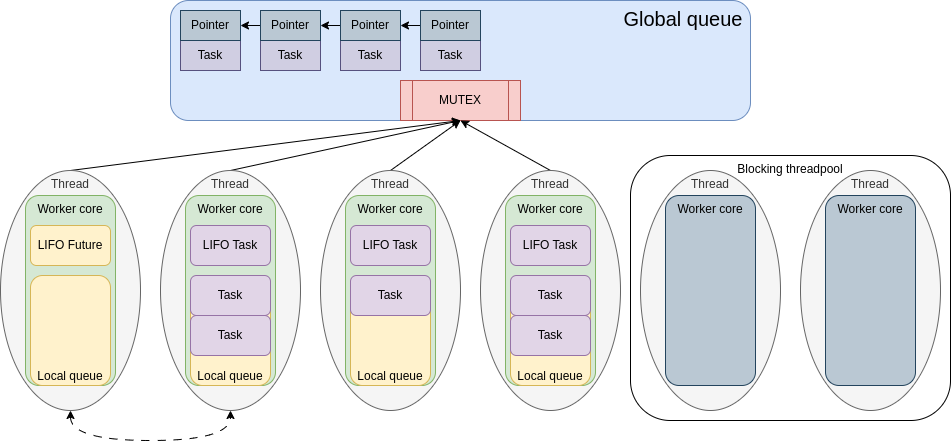
\includegraphics[scale=0.35]{pictures/tokio.arch.png}}
    \end{center}

    \caption{Упрощенное представление многопоточного рантайма}
    \label{fig:tokio:arch}
\end{figure}

\end{frame}

\begin{frame}
  \frametitle{Постановка задачи}
  \textbf{Целью} работы является проверка и решение проблемы глобальной очереди

  \textbf{Задачи}:
  \begin{itemize}
    \item Произвести обзор и выработку метрик
    \item Создать воспроизводимую систему бенчмарков
    \item Произвести анализ собранных метрик
    \item Спроектировать решение
    \item Прототипировать и анализировать полученные решения
    \item Интегрировать решение.
  \end{itemize}
\end{frame}

\begin{frame}
\frametitle{Метрики}
  \begin{itemize}
    \item Семплирование
    \begin{itemize}
      \item tokio-metrics\footnote{\href{https://github.com/tokio-rs/tokio-metrics}{Репозиторий} проекта tokio-metrics (Дата обращения: 4.1.2025)}
    \end{itemize}
    \item Тотальная оценка
    \item Выработка
    \begin{itemize}
      \item global\_queue\_depth
      \item total\_overflow\_count
      \item total\_local\_queue\_depth
      \item num\_remote\_schedules
      \item total\_steal\_operations
      \item num\_alive\_tasks
      \item poll\_time\_histogram\_bucket\_range
    \end{itemize}
  \end{itemize}
\end{frame}

\begin{frame}[fragile]
  \frametitle{Система бенчмарков}
  \begin{itemize}
    \item \verb|tokiobench|\footnote{\href{https://github.com/IgorErin/tokiobench}{Репозиторий} проект tokiobench (Дата обращения: 4.1.2025)} --- проект с бенчмарками
    \begin{itemize}
    \item Сценарии интересные потребителю
    \item Сбор метрик
    \item Визуализация
    \end{itemize}
    \item Поиск сценария
    \begin{itemize}
      \item Репозиторий tokio
      \item Обсуждение с потребителями
    \end{itemize}
    \item Проблема синхронизации
    \begin{itemize}
      \item Атомарные бенчмарки в tokio
      \item \verb|block_on|
    \end{itemize}
  \end{itemize}
\end{frame}


\begin{frame}[fragile]
  \frametitle{Проблема синхронизации 1}
    \begin{minted}{rust}
for _ in 0..NUM_SPAWN {
    handles.push(rt.spawn(async {}));
}
rt.block_on(async {
    for handle in handles.drain(..) {
        handle.await.unwrap();
    }
});
    \end{minted}

\end{frame}

\begin{frame}[fragile]
  \frametitle{Проблема синхронизации 2}
    \begin{minted}{rust}
let (tx, rx) = mpsc::sync_channel(1000);
let rem = Arc::new(AtomicUsize::new(NUM_SPAWN));
rt.block_on(async {
    for _ in 0..NUM_SPAWN {
        let tx = tx.clone();
        let rem = rem.clone();
        tokio::spawn(async move {
            if 1 == rem.fetch_sub(1, Relaxed) {
                tx.send(()); // send signal
            }
        });
    }
    rx.recv(); // block benchmark thread until signal
});
    \end{minted}
\end{frame}


\begin{frame}[fragile]
  \frametitle{Экспериментальное исследование}
  Постановка эксперимента
  \begin{itemize}
    \item criterion --- бенчмарк фреимворк
    \item Спавнер
    \begin{itemize}
      \item Создатель большого количества задач
      \item В блокирующем потоке
    \end{itemize}
    \item Листовые задачи
    \begin{itemize}
      \item Пустые асинхронные замыкания
      \item Непрозрачные для компилятор
    \end{itemize}
    \item Система
    \begin{itemize}
      \item YADRO VEGMAN Rx20 G2\footnote{\href{https://yadro.com/ru/vegman/rx20g2/specs}{Официальные} характеристики системы}
    \end{itemize}
    \item Среднее отклонение не привысило 3 процентов
  \end{itemize}
\end{frame}

\begin{frame}[fragile]
  \frametitle{Пропусная способность 1}

  \begin{center}
    \makebox[\textwidth]{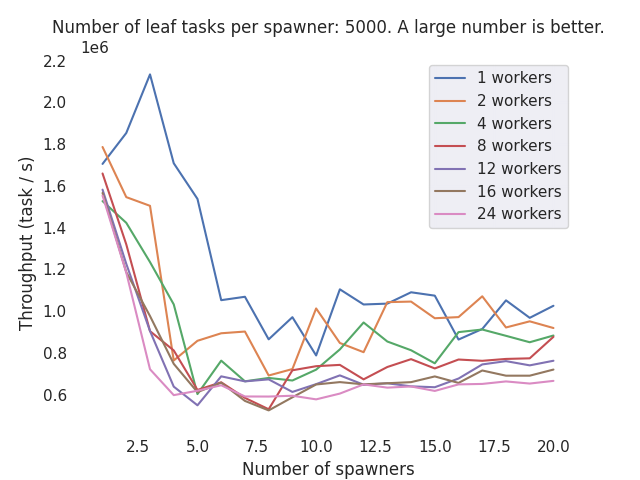
\includegraphics[scale=0.60]{pictures/tatlin_blocking.png}}
  \end{center}
\end{frame}

\begin{frame}[fragile]
  \frametitle{Пропусная способность 2}

  \begin{center}
    \makebox[\textwidth]{\includegraphics[scale=0.60]{pictures/tatlin_blocking_from_8.png}}
  \end{center}
\end{frame}

\begin{frame}[fragile]
  \frametitle{Пропусная способность}

  \begin{center}
    \makebox[\textwidth]{\includegraphics[scale=0.35]{pictures/steal_worker.png}}
  \end{center}
\end{frame}

\begin{frame}[fragile]
  \frametitle{Результаты}
  \begin{itemize}
    \item Произведен обзор метрик
    \begin{itemize}
      \item Выбраны основные
    \end{itemize}
    \item Создана система бенчмарков \verb|tokiobench|\footnote{\href{https://github.com/IgorErin/tokiobench}{Репозиторий} проекта tokiobench (Дата обращения: 4.1.2025)}
    \item Произведен анализ полученные результатов
    \item Проектирование
    \begin{itemize}
      \item Не найдены изменения в Go рантайме
    \end{itemize}
  \end{itemize}
\end{frame}

%\addtocounter{framenumber}{1}
\appendix

\end{document}
